\chapter{Evaluation}
\section{Correctness} 
For correctness, we create two virtual topologies : Vt1($h1,h2,h3$) and Vt2($h4,h5,h6$). Hosts in Vt1 and Vt2 must be able to talk to each other. And, since tenants are \emph{isolated} from each other, hosts of Vt1 should not be able to talk to Vt2 and vice-versa. The results of a \verb|pingall| operation in Mininet gives the following results, thus verifying correctness.
\begin{verbatim}
	> pingall
	h1 -> h2 h3 X X X
	h2 -> h1 h3 X X X
	h3 -> h1 h2 X X X
	h4 -> X X X h5 h6
	h5 -> X X X h4 h6
	h6 -> X X X h4 h5
\end{verbatim}
\section{Virtual Topology Mapping}
We create a \verb|TopologyCreator| class to create ring and tree topologies of custom length and depth respectively. To analyse the time complexity of mapping the virtual topology onto the physical topology, we create a tree topology of depth 10 as our physical topology and map virtual topologies of varying size and measure the time taken for the mapping. As we can observe in Figure 6.1 and 6.2, the time taken to calculate the mapping is constant across different virtual topologies(and less than 0.1 of a second). This follows from the algorithm as well, as the time complexity depends on the size of the physical topology.
\begin{figure}
	\noindent
	\makebox[\textwidth]{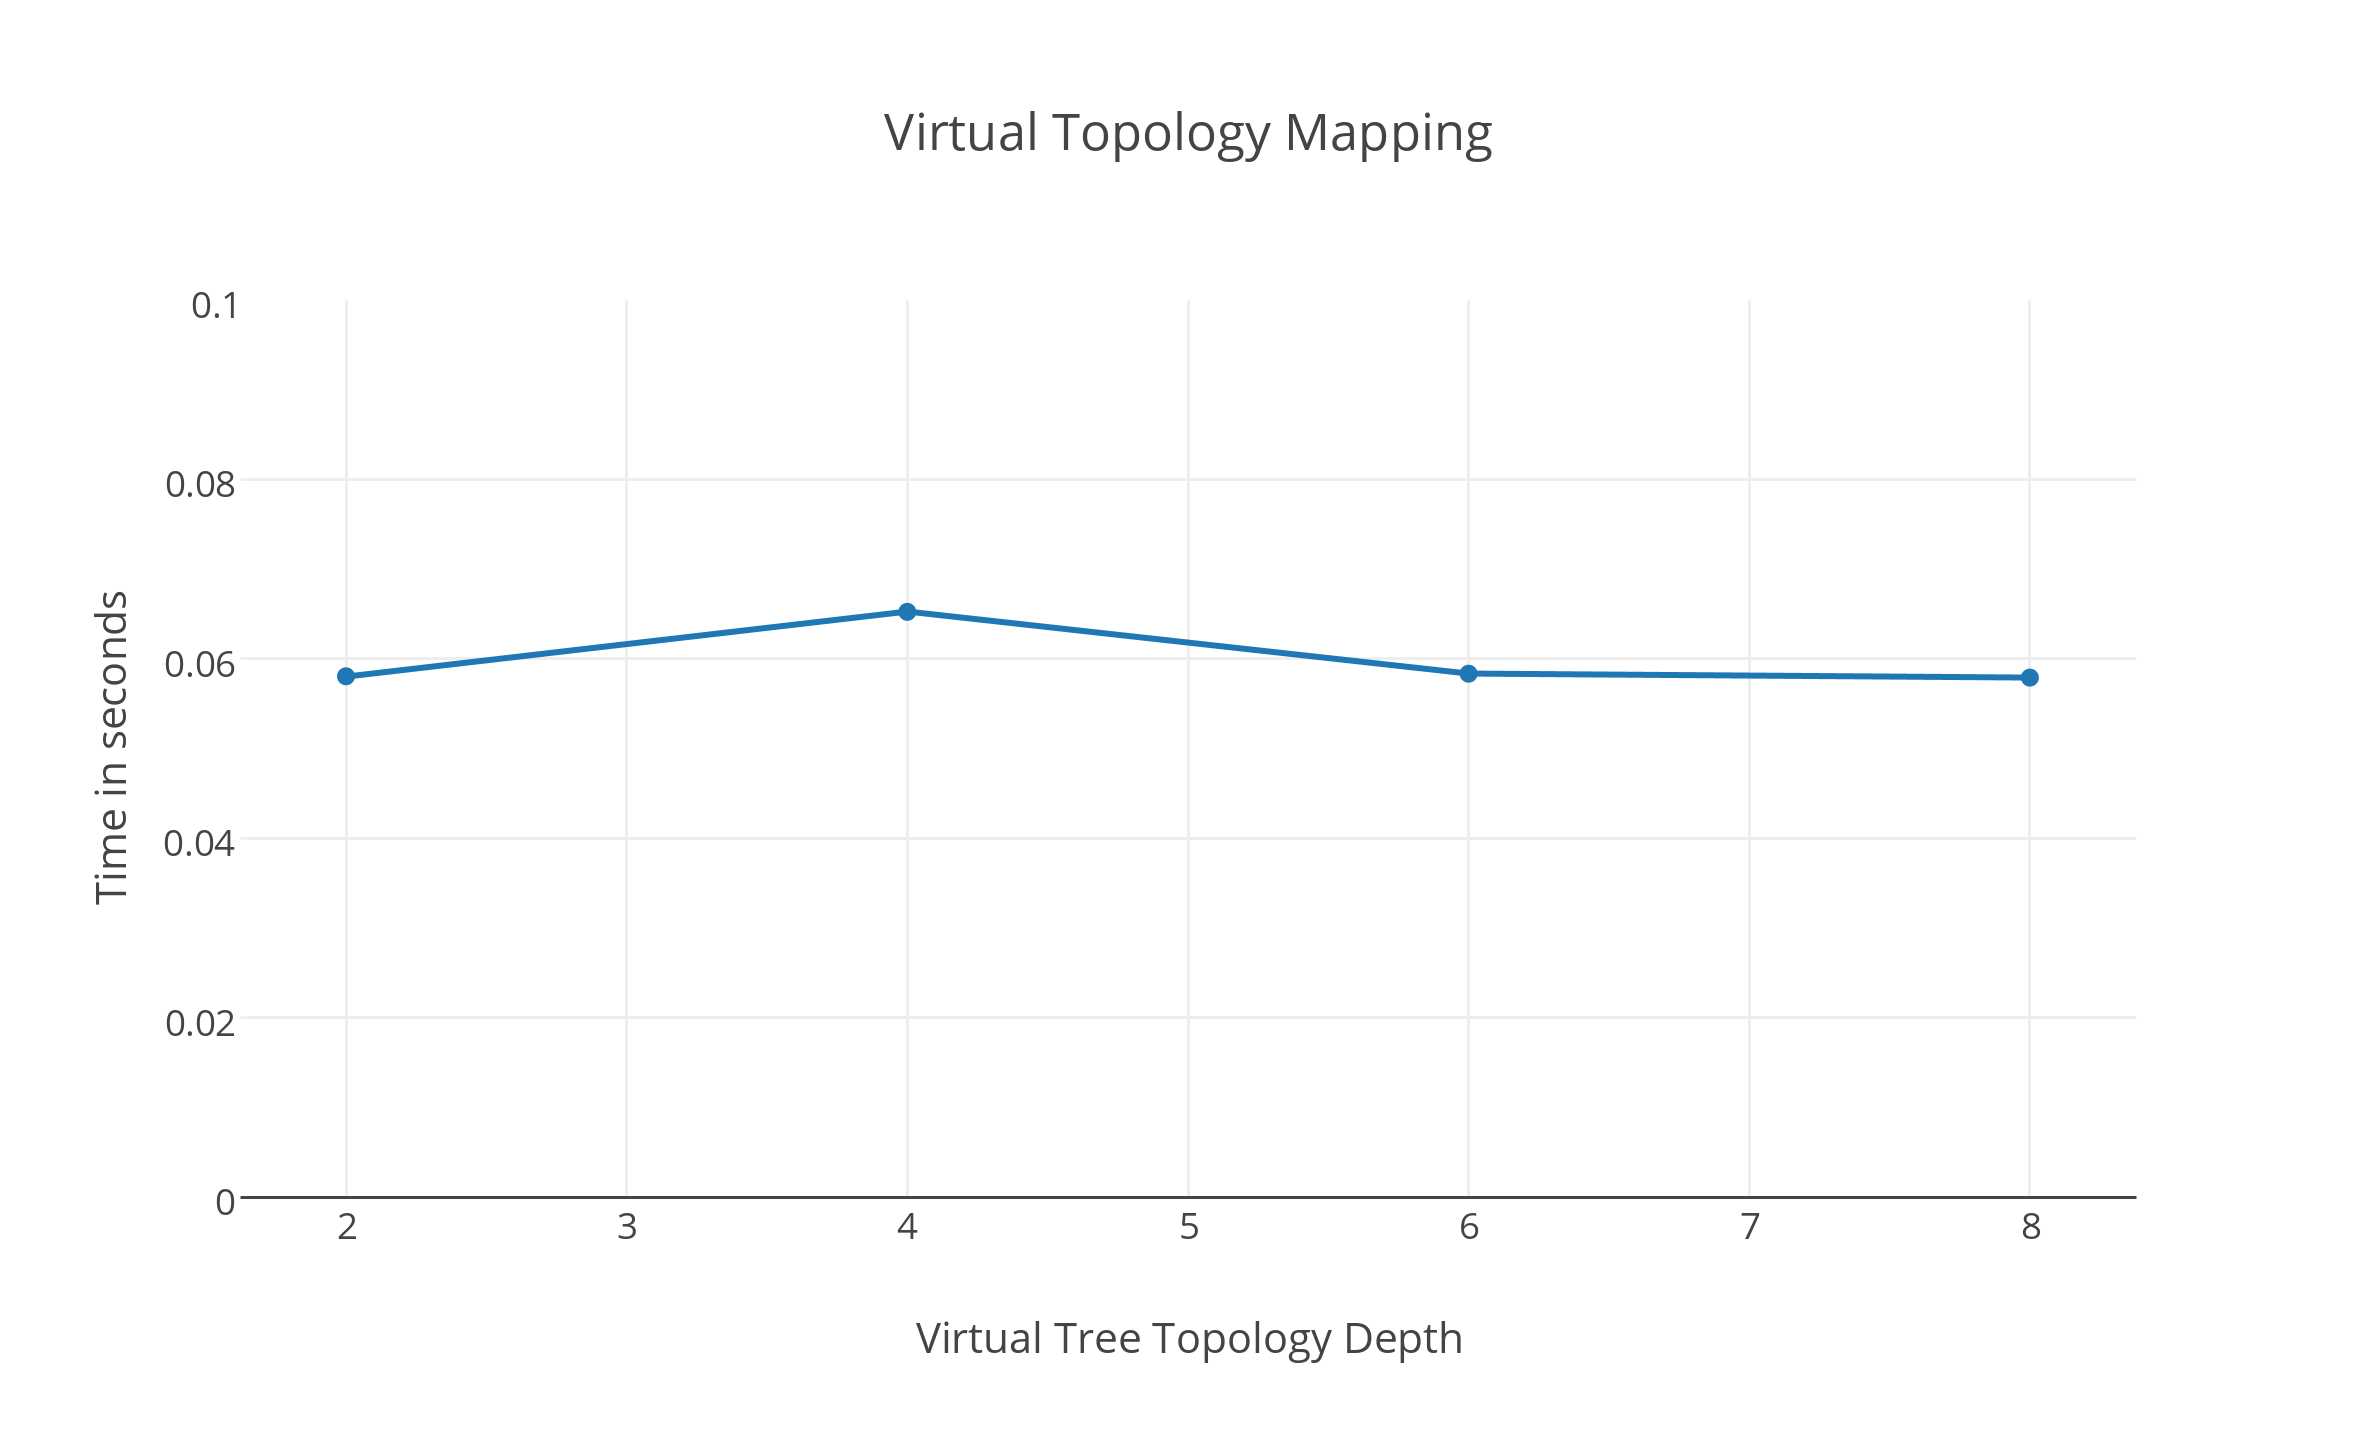
\includegraphics[width=15cm]{Figures/vtmt.png}}%
	\caption{Virtual Topology Mapping for varying tree topologies}
\end{figure}

\begin{figure}
	\noindent
	\makebox[\textwidth]{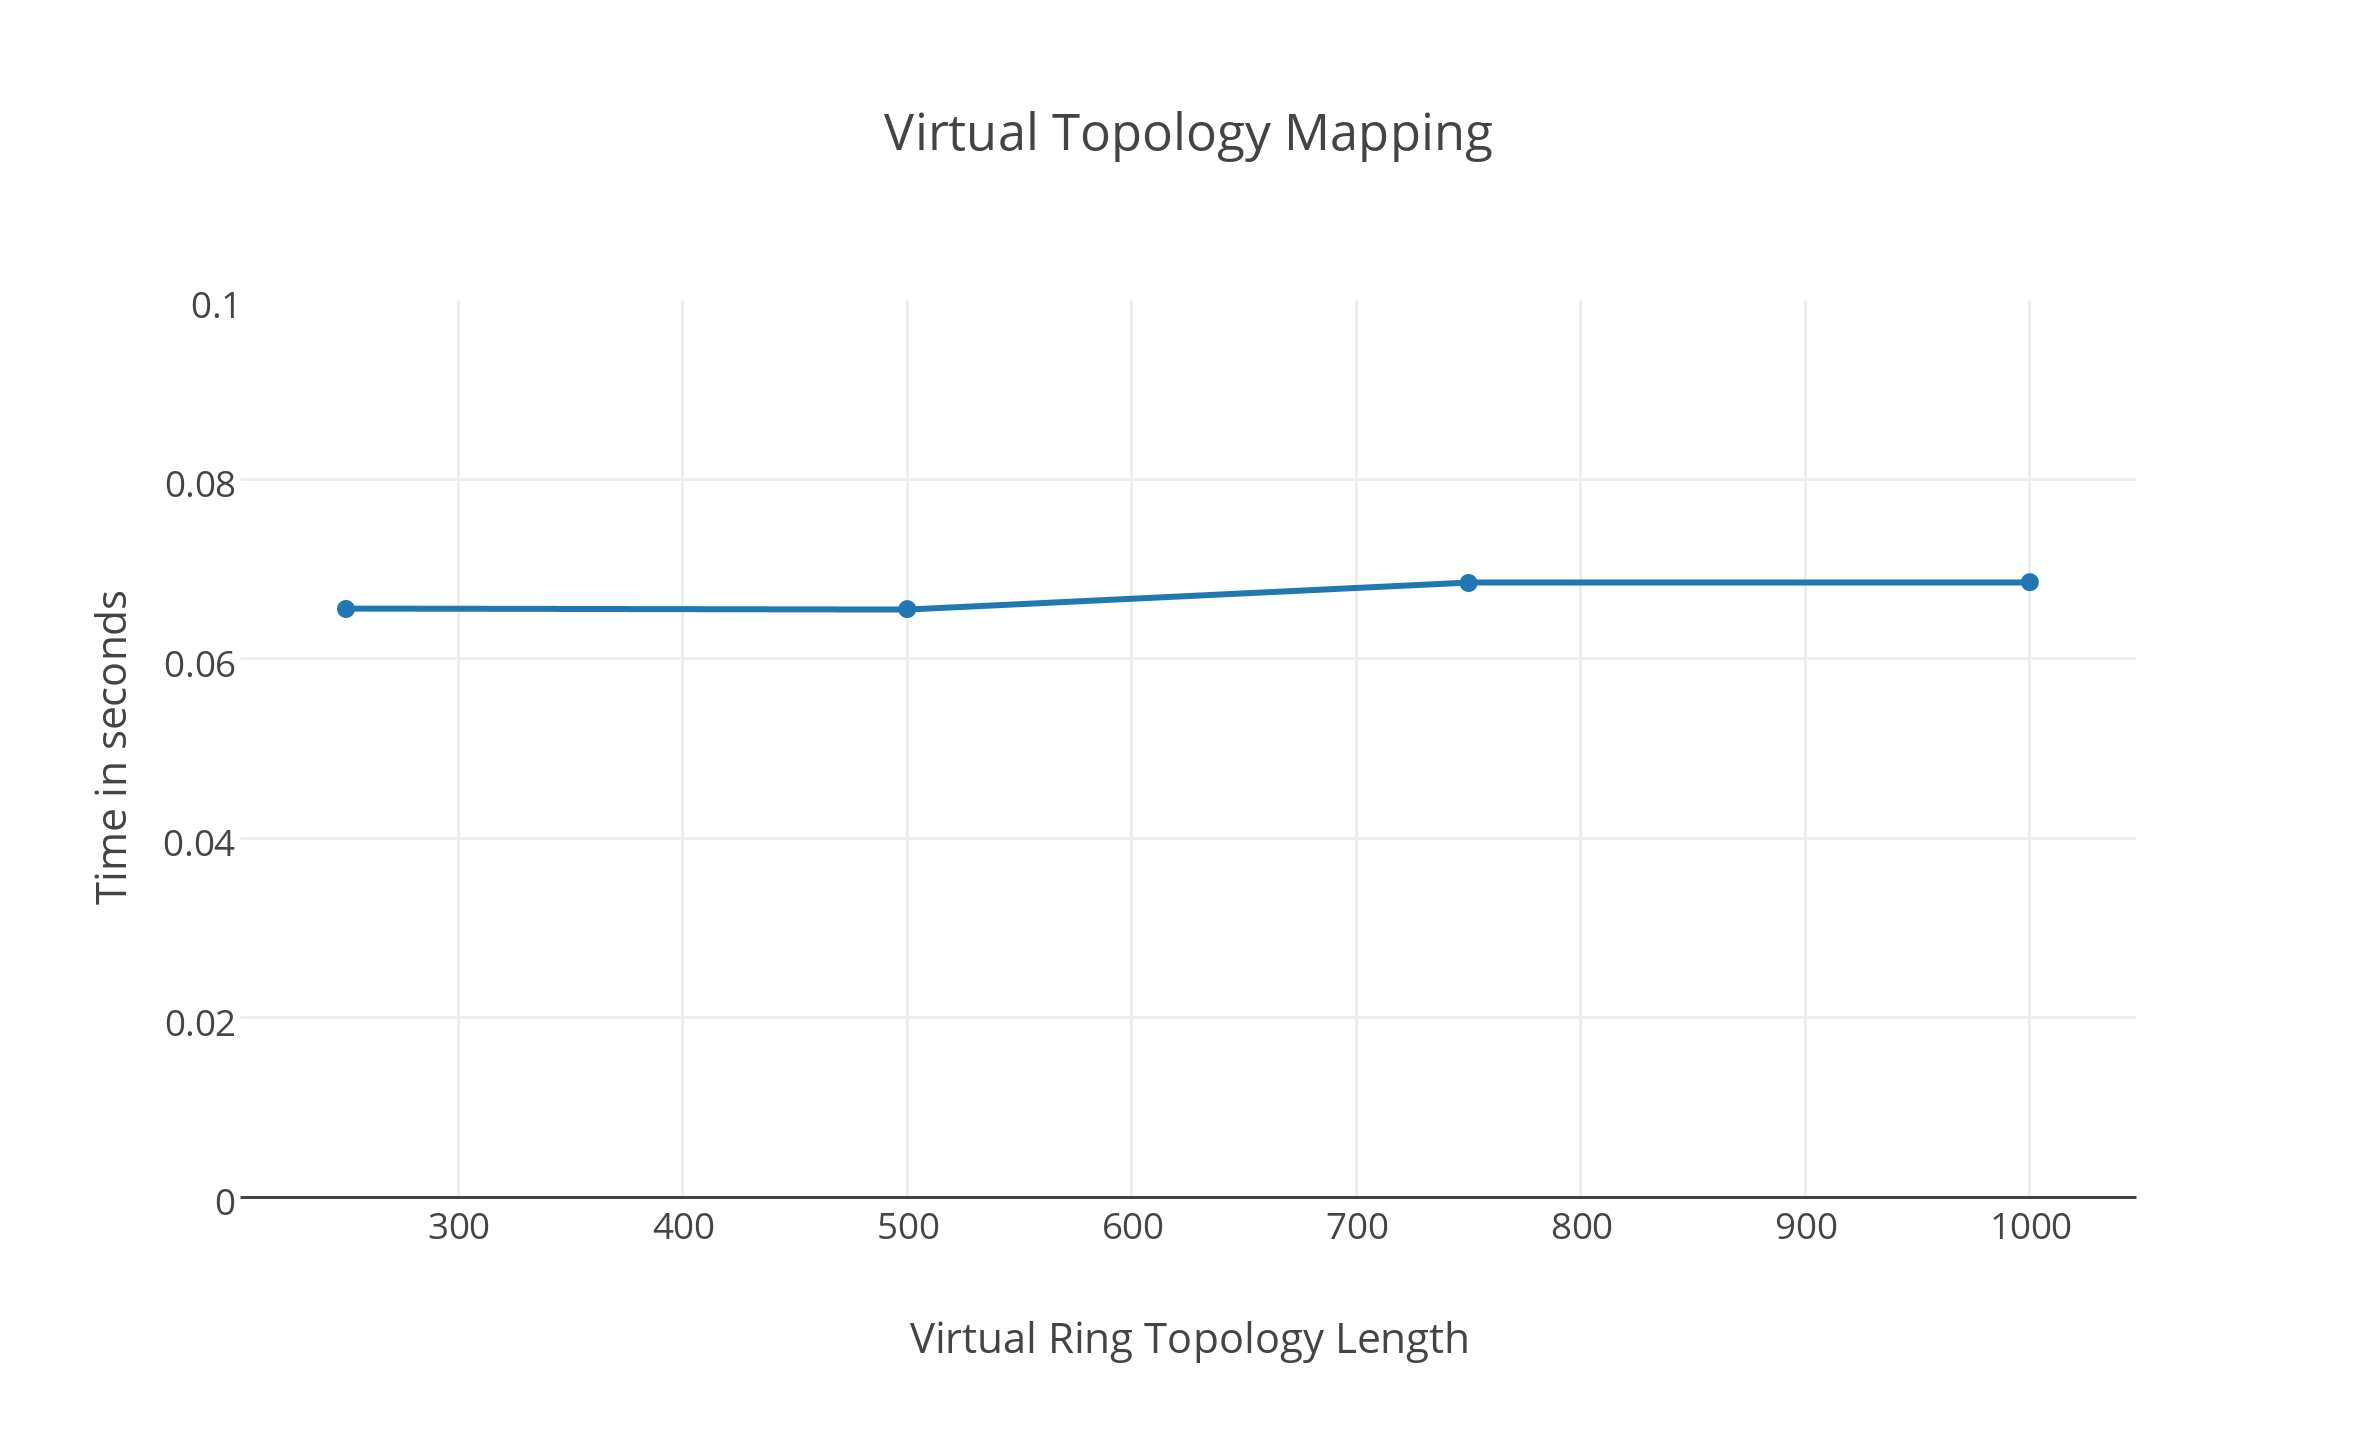
\includegraphics[width=15cm]{Figures/vmtr.png}}%
	\caption{Virtual Topology Mapping for varying ring topologies}
\end{figure}

\section{Network Route Calculation}
The next step is to calculate the \emph{complete} network routes between every pair of hosts in the virtual topology. We can infer that this time will be dependent on the sizes of both the virtual topology and physical topologies and the mapping heuristic used. Since we try to minimise the diameter of the mapped virtual network graph, we would obtain better results than other mapping schemes. The physical topology is a tree topology of depth 10 and we vary the mapped virtual topology sizes. Figures 6.3 and 6.4 plot the time taken to calculate the network routes for the varying virtual topologies. 

\begin{figure}
	\noindent
	\makebox[\textwidth]{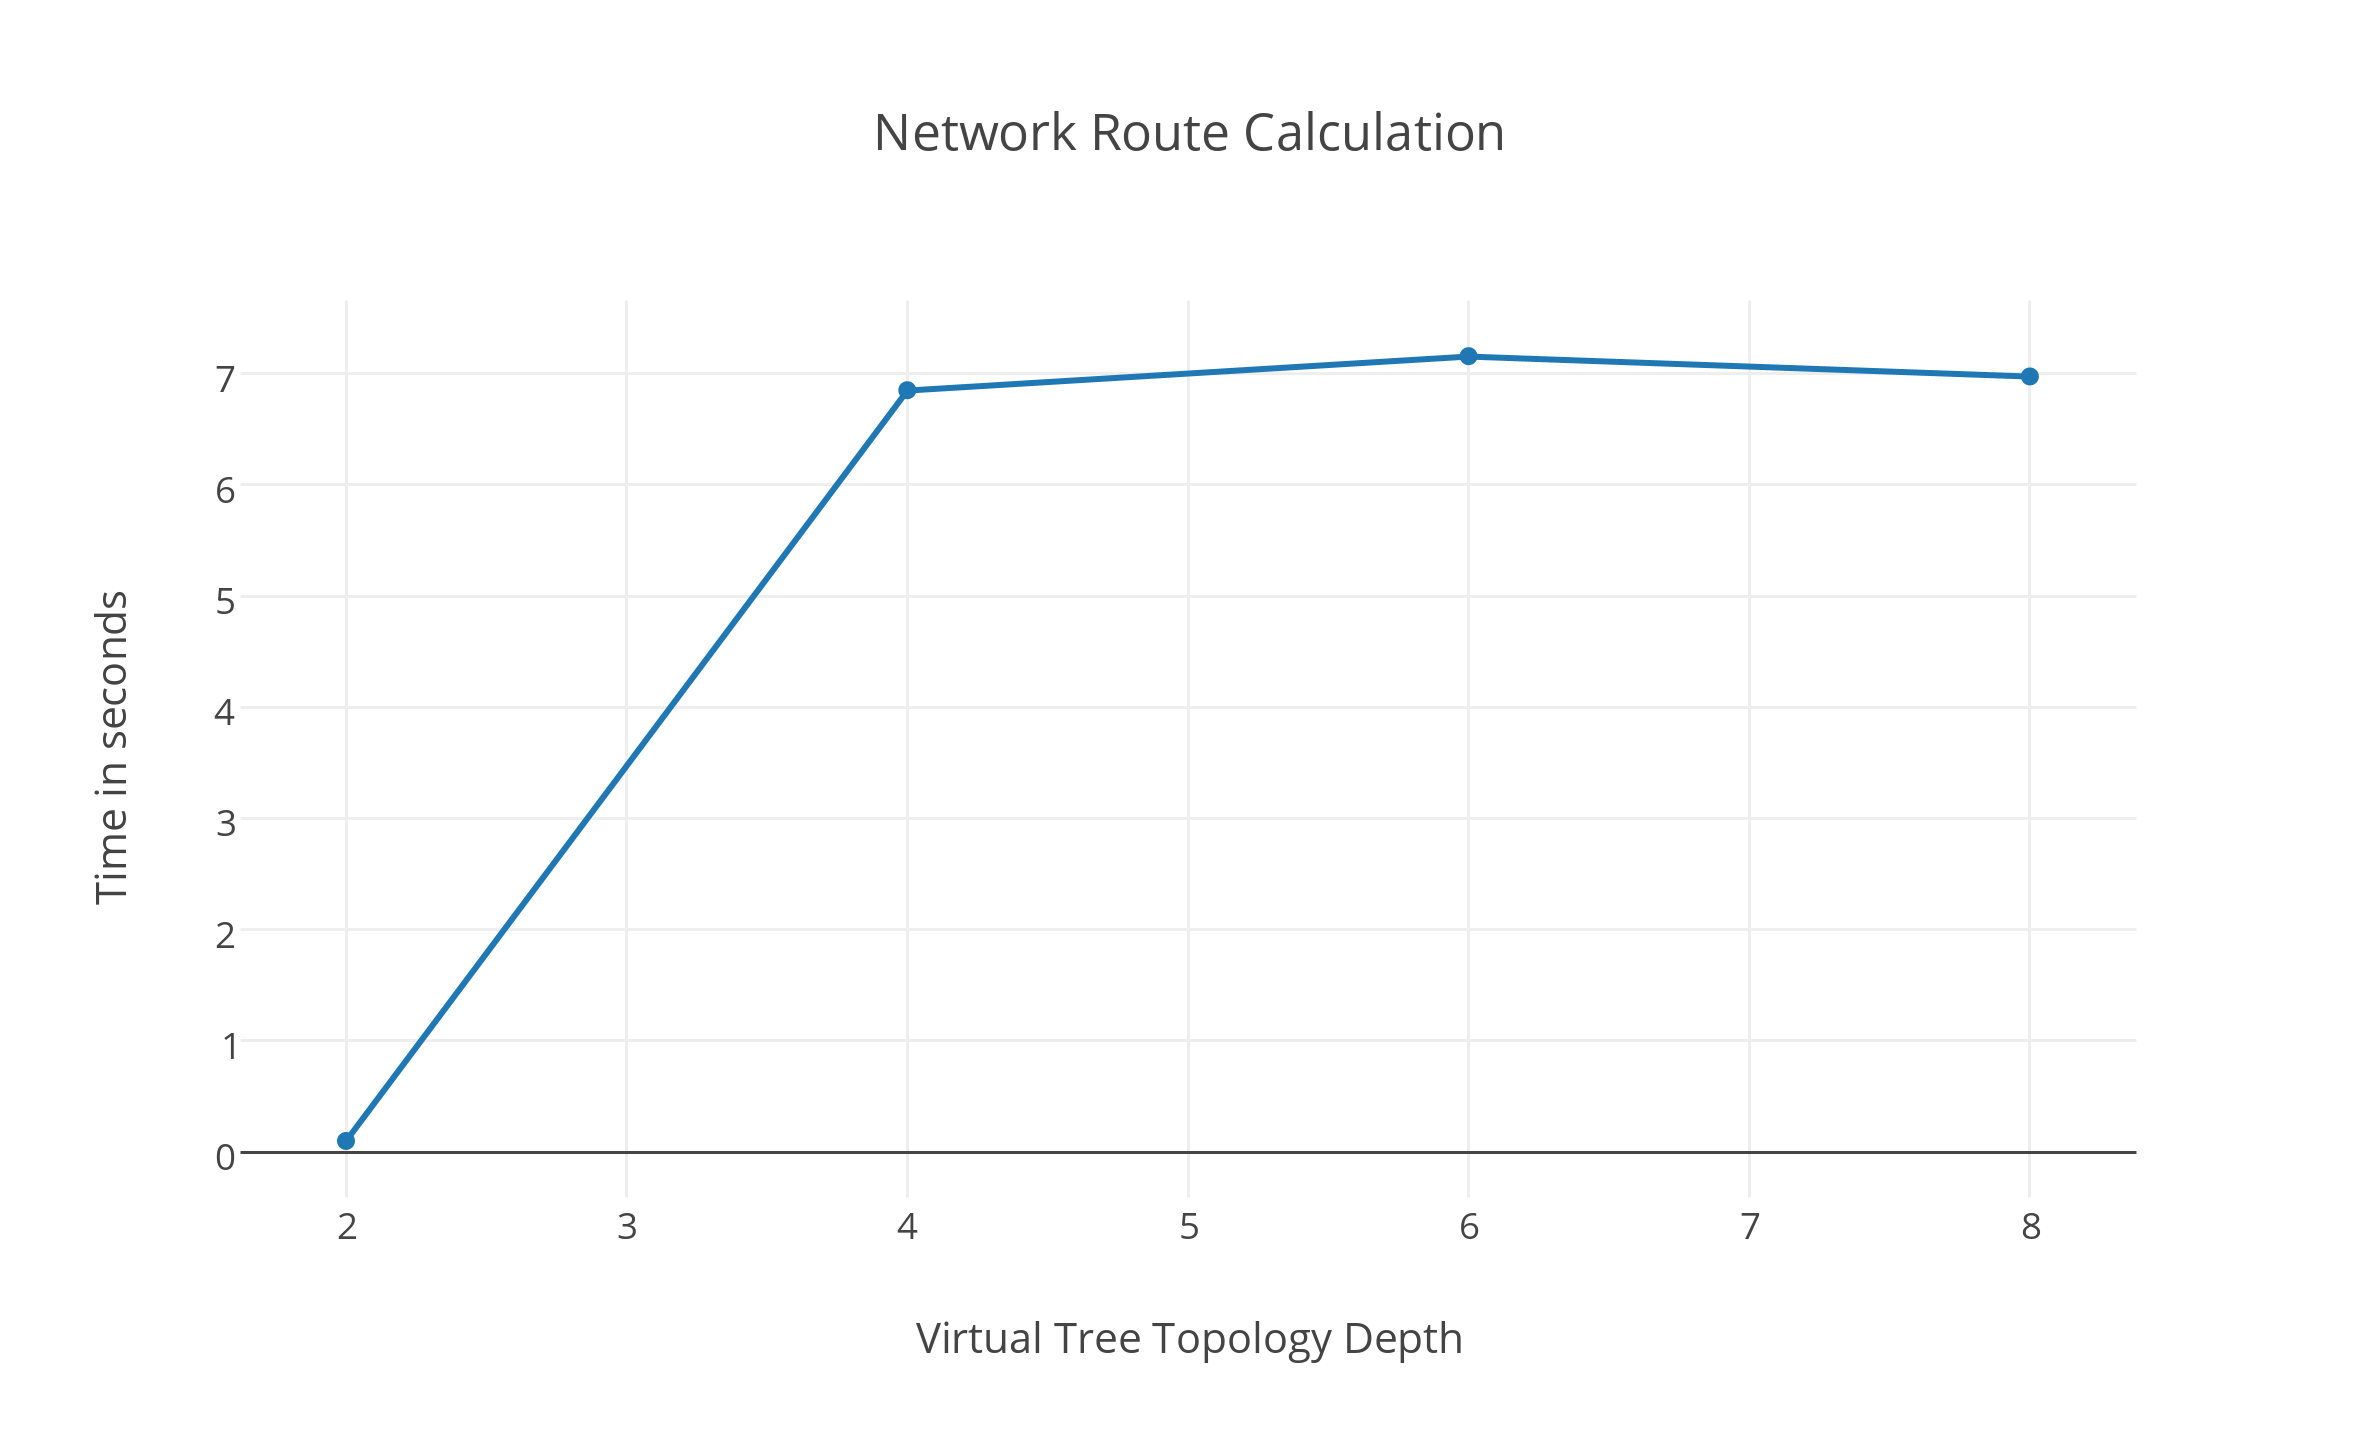
\includegraphics[width=15cm]{Figures/nrt.png}}%
	\caption{Network Route Calculation for varying tree topologies}
\end{figure}

\begin{figure}
	\noindent
	\makebox[\textwidth]{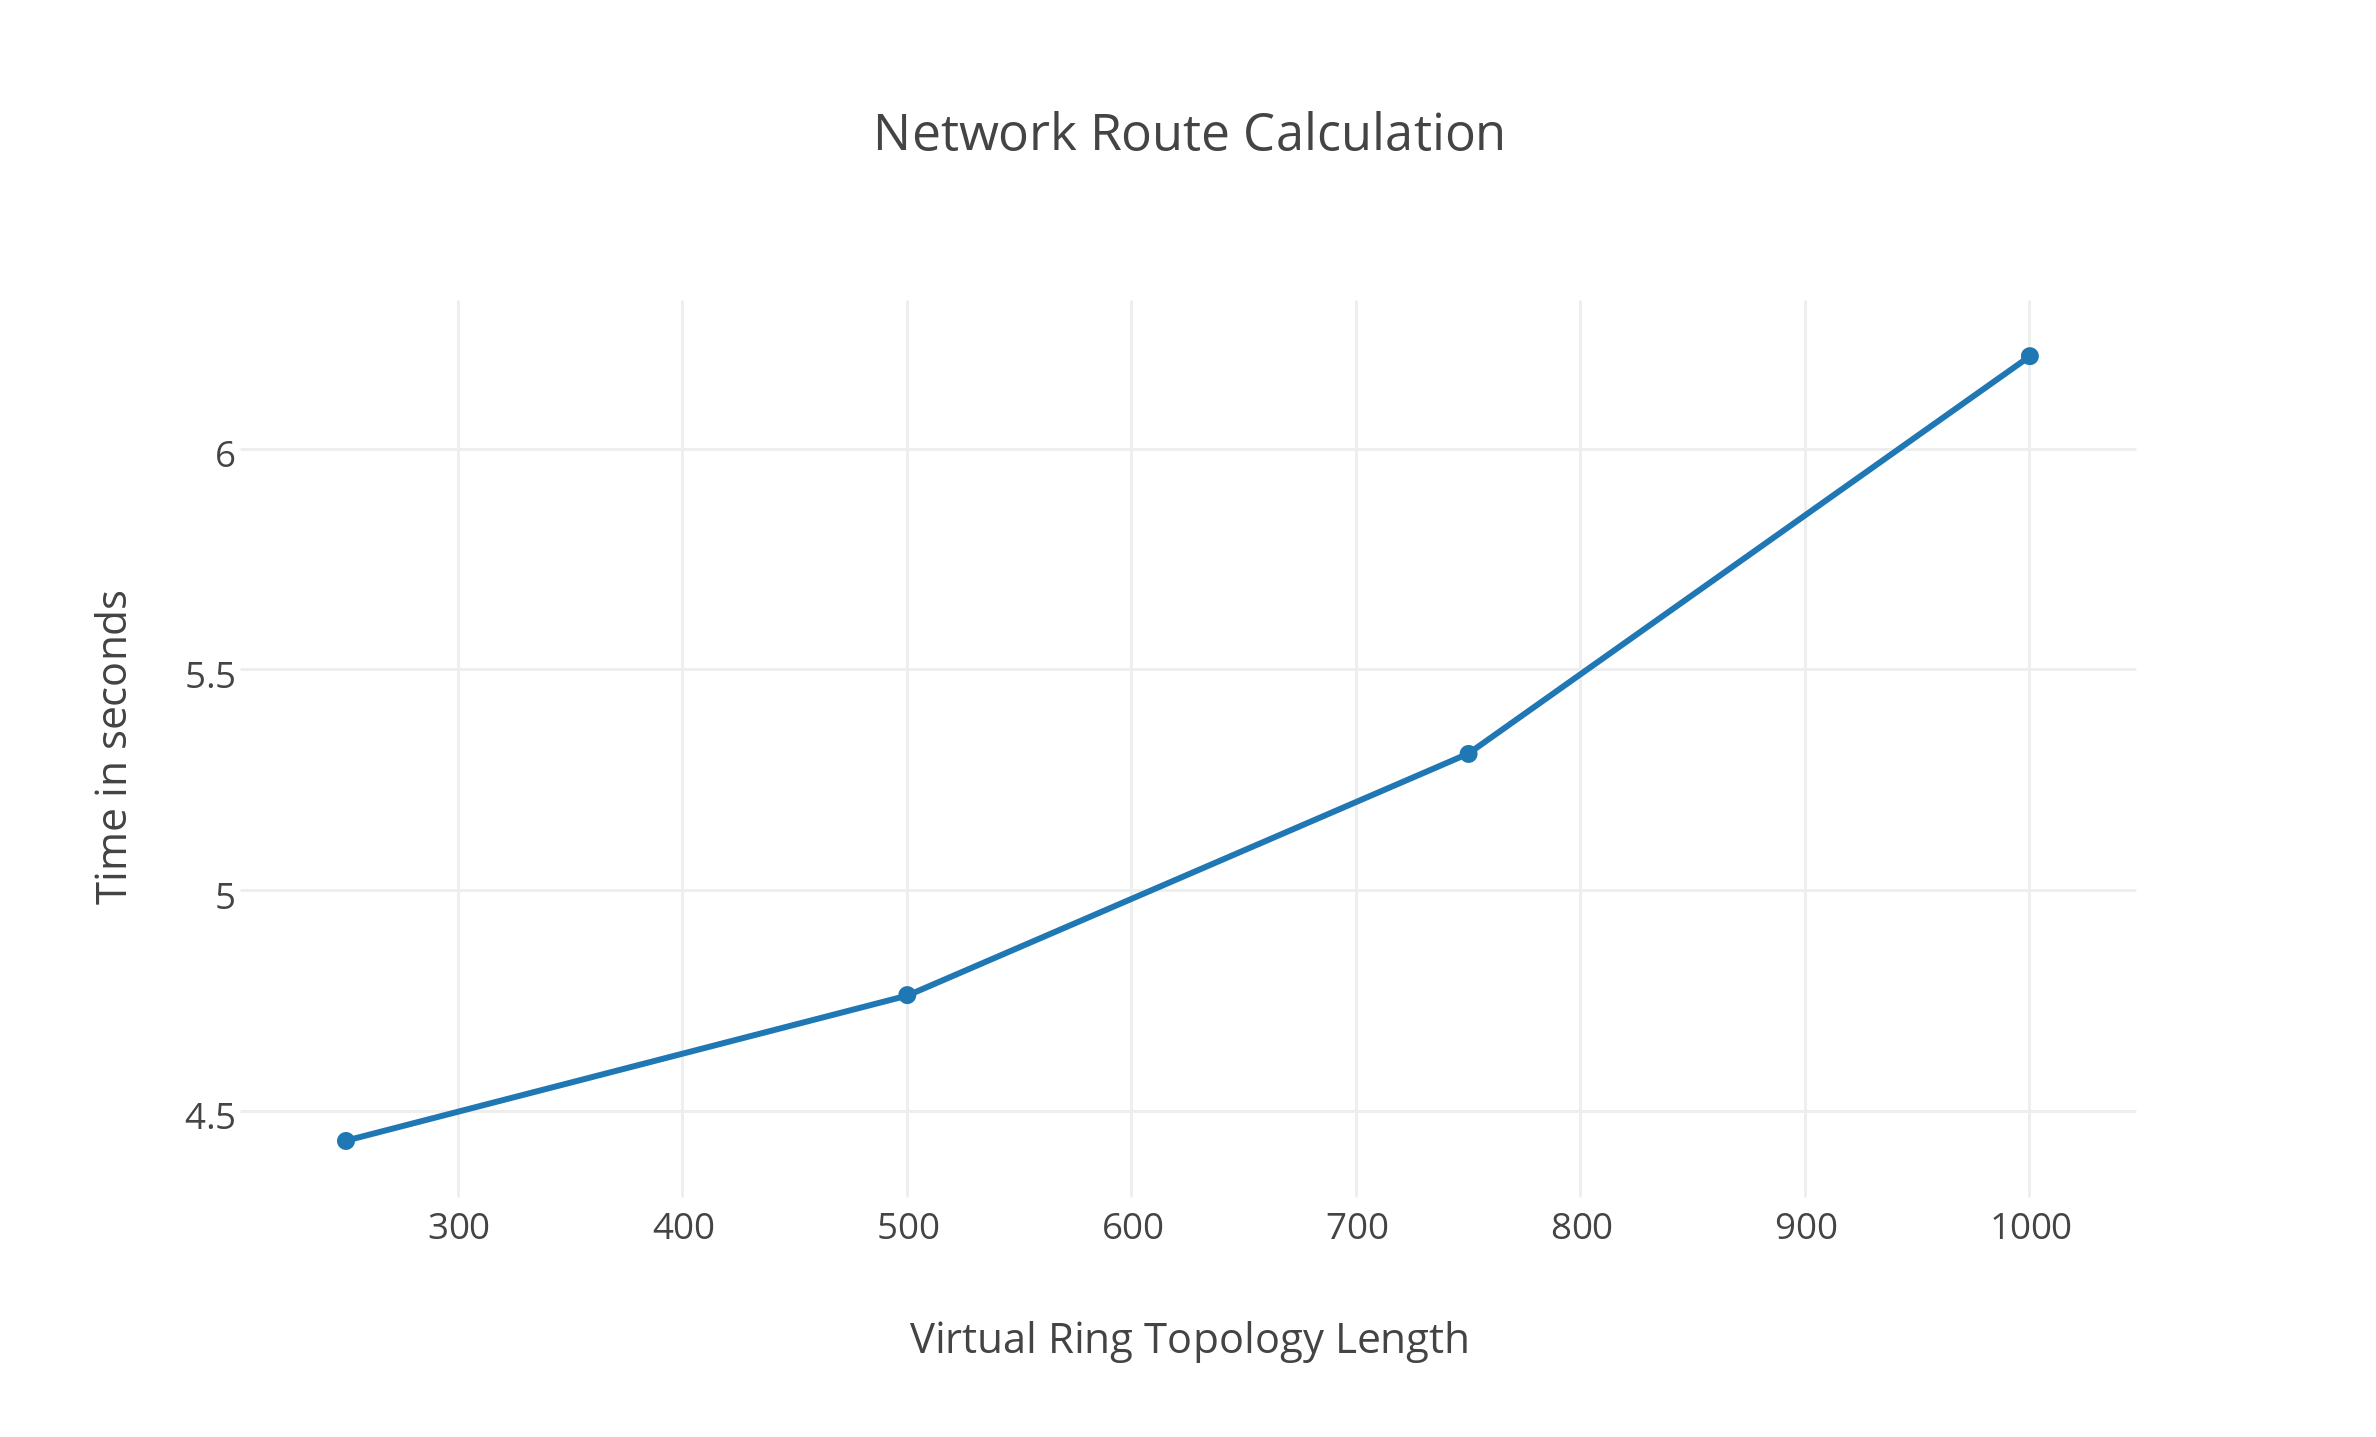
\includegraphics[width=15cm]{Figures/nrr.png}}%
	\caption{Network Route Calculation for varying ring topologies}
\end{figure}
